\documentclass[conference]{IEEEtran}
\IEEEoverridecommandlockouts

% ---------- packages ----------
\usepackage[T1]{fontenc}
\usepackage[utf8]{inputenc}
\usepackage{amsmath,amssymb,amsfonts}
\usepackage{graphicx}
\usepackage{booktabs}
\usepackage{array}
\usepackage{url}
\usepackage{xcolor}
\usepackage{listings}
\usepackage{tikz}
\usetikzlibrary{arrows.meta,positioning,fit,backgrounds}
\usepackage[hidelinks]{hyperref}
\usepackage{cleveref}
% ---------- compactness (fit to 6 pages; spacing only, no wording change) ----------
\usepackage{enumitem}
\setlist[itemize]{topsep=2pt,itemsep=1pt,parsep=0pt,partopsep=0pt,leftmargin=1.35em}
\setlength{\textfloatsep}{6pt plus 2pt minus 2pt}
\setlength{\dbltextfloatsep}{7pt plus 2pt minus 2pt}
\setlength{\floatsep}{6pt plus 2pt minus 2pt}
\setlength{\intextsep}{6pt plus 2pt minus 2pt}

% ---------- listing style ----------
\definecolor{codebg}{rgb}{0.965,0.965,0.965}
\lstset{
  basicstyle=\ttfamily\scriptsize,
  backgroundcolor=\color{codebg},
  breaklines=true,
  columns=fullflexible,
  frame=single,
  framesep=3pt,
  showstringspaces=false,
  keepspaces=true,
  abovecaptionskip=3pt,
  belowcaptionskip=4pt
}

\newcommand{\rg}{\textsc{ReasonGuard}}

\begin{document}

\title{\rg: Verifiable Guardrails for Natural-Language Explanations\\ from Formal Anomaly Detectors in Safety-Critical Systems}

\author{\IEEEauthorblockN{Ravan Bilalov}
\IEEEauthorblockA{M.Sc. Applied Data Science and Analytics\\
SRH University Hamburg, Germany\\
in collaboration with the Faculty of Information Technology,\\
Brno University of Technology (NES@FIT), Czech Republic\\
\texttt{ravanbilalov03@gmail.com}}}

\maketitle

% ============================================================
\begin{abstract}
Large Language Models (LLMs) are increasingly used to turn machine-readable outputs from formal anomaly detectors into natural-language explanations. These explanations can be hallucinated or otherwise unfaithful to the detector's actual verdict, potentially misleading human operators. We propose \rg, a runtime verifier that enforces machine-checkable faithfulness criteria on explanations of detector verdicts, defined over a specification of the monitored property. \rg{} is deterministic, auditable, and fail-closed, enabling safe deployment of LLM-generated explanations in safety-critical settings. We apply \rg{} in the context of anomaly detection on private network tele-control traffic from an electrical substation conforming to the IEC-104 protocol. We present a taxonomy of faithfulness violations, provide a formalization of each violation class along with the corresponding violation-detection rule, and give actionable explanations of violations.

We demonstrate \rg's applicability on a corpus of 500 LLM-generated explanations of detector verdicts on smart-grid network traffic from Brno University of Technology, comprising outputs from three locally-run LLMs and two cloud-based LLMs, and 500 synthetic explanations crafted to induce known violations as regression test cases. We provide a benchmark of 200 ground-truth annotations produced by human annotators. \rg{} flags violations with varying reliability: for example, it detects fabricated entities with precision of 0.90 but only recall of 0.09, and under-specification with precision of 0.48 and recall of 0.92. We find statistically significant associations between violation occurrence and the LLM used to generate explanations as well as the type of event being explained. \rg{} has limited agreement with human-generated annotations ($\kappa = 0.16$), primarily due to overly permissive criteria resulting in overtriggering, indicating its applicability in human-in-the-loop settings. \rg's fine-grained violation classes (five in total, referred to as V1--V5), actionable explanations of violations, and fail-closed design enable human-in-the-loop use-cases by prioritizing explanations for human review, and map to Article~13 (transparency) and Article~17 (quality management) of the EU AI Act. We release our implementation, prompts, and datasets under an open-source license.
\end{abstract}

\begin{IEEEkeywords}
runtime verification, faithfulness, large language models, formal methods, industrial control systems, IEC-104, EU AI Act, explainability
\end{IEEEkeywords}

% ============================================================
\section{Introduction}\label{sec:intro}

Large language models (LLMs) can be used to generate natural-language explanations of data or predictions, making them attractive in high-stakes domains where decisions made on the basis of that data need to be auditable and comprehensible to domain experts. One such domain is cybersecurity. Existing work on runtime verification for industrial control systems uses finite-state automata that formally model the specification of correct behavior in private tele-control networks connecting substations in a smart-grid. These monitors observe traffic conforming to the IEC-104 protocol in real time, and raise an alarm with a certificate, that is, a proof, of the specification violation that can indicate a network attack. Operators can be alerted about attacks by viewing the verdicts of such anomaly-detection programs. However, the verdicts themselves can be difficult to understand, making it challenging for operators to act upon them in a timely fashion. Recent work has explored using LLMs to generate natural-language explanations of verdicts raised by such programs. In critical use-cases such as monitoring for network attacks, it is paramount that these explanations are faithful to the verdicts raised by these programs, as false positives could result in wasted effort and false negatives could result in real attacks going unnoticed.

Standard methods of evaluating LLM-generated explanations operate offline on a set of inputs~\cite{Maynez2020Faithfulness,Min2023FActScore,Honovich2022True}. In contrast, in order to safely deploy such explanations we seek guarantees about the faithfulness of any individual explanation generated in response to any individual input from the anomaly detector at runtime. This motivates the use of runtime verification to enforce criteria that any LLM-generated explanation must satisfy. We propose \rg, a framework that uses runtime verification to provide machine-checkable guarantees about the faithfulness of LLM-generated natural-language explanations of verdicts from anomaly-detection programs. \rg{} takes a specification of the property being monitored by the anomaly-detection program along with the verdict raised by the program on the monitored system, and verifies whether the LLM-generated explanation adheres to criteria for being faithful to the verdict. \rg{} raises alarms in case of unfaithfulness with actionable explanations.

\noindent\textbf{Contributions.}
First, we propose \rg, a novel, deterministic, auditable, and fail-closed verifier that checks whether LLM-generated, natural-language explanations of formal verification results are faithful to the results. We instantiate it for checking explanations of outputs from an anomaly detector for the IEC-104 industrial control system communication protocol (\cref{sec:framework}).

Second, we conduct an extensive empirical study of \rg{}, including:
\begin{itemize}
  \item a dataset of 500 LLM-generated explanations of IEC-104 detector verdicts using three local and two cloud-based LLMs;
  \item a suite of 500 synthetic test cases for regression-testing \rg{} and a benchmark of 200 blind ground-truth annotations;
  \item evidence for a statistically significant association between the faithfulness violations flagged by \rg{} and both the model that produced the explanation and the event being explained;
  \item a discussion of false alarms, and of using \rg{} in the loop with a human analyst as a triage tool;
  \item a mapping of \rg{} to Articles~13 and~17 of the EU AI Act~\cite{EUAIAct2024};
  \item open-source, fully reproducible research artifacts~\cite{ReasonGuardArtifact2026}.
\end{itemize}

Third, we introduce a taxonomy of types of unfaithfulness in LLM-generated natural-language explanations of anomaly-detection results, along with rules to detect these types and an indication of their severity for prioritizing analyst attention.

\section{Background and Related Work}\label{sec:related}

\subsection{Formal methods and automaton-based ICS detection}
Model checking is a formal verification technique that determines whether a given model of a finite-state system fulfills some specification formulated in some temporal logic~\cite{ClarkeModelChecking2001}. In the context of ICSs, the specification describes the system's legitimate behavior. Observing a violation of the specification thus gives a definite indication that an anomaly has occurred with respect to the system's model. Havlena et al.~\cite{HavlenaMatousekRysavyHolik2023} infer a deterministic probabilistic automaton using legitimate IEC-104 and MMS traffic. They also take into account the semantics of the messages, reducing false positives. The resulting anomaly detector produces a structured verdict describing the nature of the anomaly, which devices were involved, when it started, etc. This verdict is used by \rg{} as an inviolable specification for its explanations.

Due to the sensitivity of LLMs to prompts and their opaque internals, it is not feasible to bound and model them like other programs and prove that their executions satisfy some property. This is where runtime verification (RV) comes in, where, instead of modeling the LLM and verifying all its executions, we verify a single execution of it.

\subsection{Faithfulness evaluation}
Faithfulness evaluation can be separated into branches: world factuality that measures whether the generation aligns with world knowledge; source faithfulness that measures whether the generation is entailed by the source~\cite{Maynez2020Faithfulness}. \textsc{FActScore}~\cite{Min2023FActScore} decomposes a given output into atomic facts and validates them with a knowledge base. \textsc{TRUE}~\cite{Honovich2022True} integrates 11 benchmarks for faithfulness evaluation and shows that natural language inference measures are complementary to question generation measures. Similar to them, \rg{} decomposes a given output into atomic claims.

Differently, we provide a deterministic and auditable process suitable for certification and propose an actionable class instead of a scalar value. Moreover, our work focuses on faithfulness to verdicts provided by formal methods, which differs from faithfulness to source documents and has received little attention.

\subsection{Runtime verification}
Runtime verification determines whether a single run of a system obeys some specification, all during execution~\cite{LeuckerSchallhart2009RuntimeVerification}. The monitor is usually generated from a specification. In our setting, the execution is the explanation, the specification is our bound and the monitor is the verifier. This correspondence is what allows us to apply runtime verification in \rg{}.

Faithfulness is a safety property since a finite input reveals whether there is a violation: a single incorrect assertion violates the specification, independent of the number of correct ones. Our bound is fail-closed since any assertion not explicitly allowed is considered incorrect. This ensures that the monitor is independent of the generator. We contribute a novel application of RV and a novel RV monitor.

\subsection{The EU AI Act}
Under the AI Act, Regulation (EU) 2024/1689~\cite{EUAIAct2024}, AI systems that are a safety component in the management and operation of essential infrastructures in the areas of electricity, gas, and water fall under high-risk systems according to Annex~III. For high-risk AI systems, providers should ensure that the systems are transparent enough for the recipients to be able to interpret and use the output appropriately under Article~13. While \rg{} is not a control component, it can help to provide evidence for fulfilling this requirement.

Furthermore, providers are expected to implement a quality-management framework under Article~17 that entails appropriate measures to monitor, document, test, and take corrective actions. \rg{} can help provide evidence for such a process by monitoring the faithfulness of the explanation shown to the operator, see \cref{sec:discussion} for more details.

% ============================================================
\section{The \rg{} Framework}\label{sec:framework}

\begin{figure*}[t]
\centering
\scalebox{0.75}{%
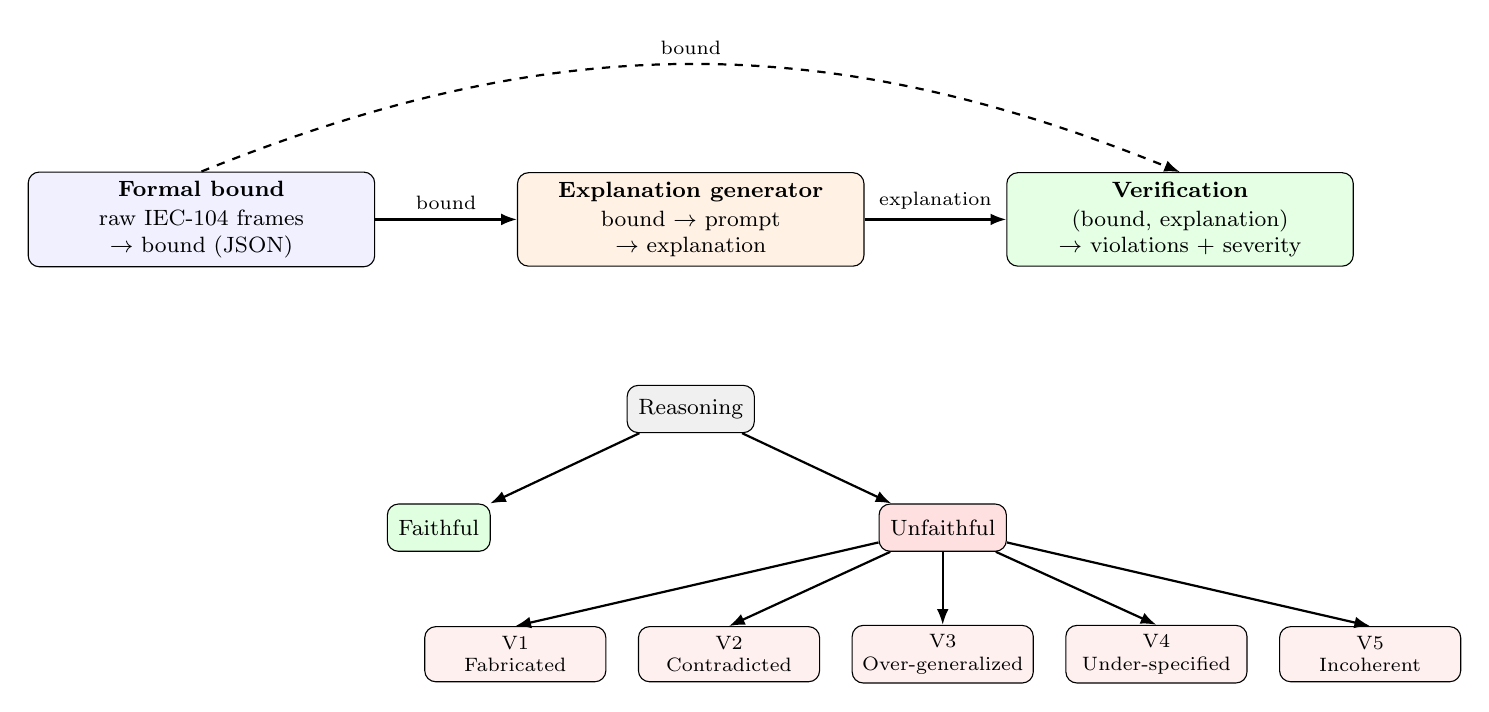
\begin{tikzpicture}[
  font=\footnotesize,
  archbox/.style={draw, rounded corners, align=center, minimum width=44mm, minimum height=10mm},
  tnode/.style={draw, rounded corners, align=center, minimum height=6mm, inner sep=4pt},
  vio/.style={draw, rounded corners, align=center, font=\scriptsize, minimum width=23mm, minimum height=7mm, fill=red!6},
  ar/.style={-{Latex[length=2mm]}, thick}
]
\node[archbox, fill=blue!6] (formal) {\textbf{Formal bound}\\[1pt] raw IEC-104 frames\\ $\rightarrow$ bound (JSON)};
\node[archbox, fill=orange!10, right=18mm of formal] (ai) {\textbf{Explanation generator}\\[1pt] bound $\rightarrow$ prompt\\ $\rightarrow$ explanation};
\node[archbox, fill=green!10, right=18mm of ai] (ver) {\textbf{Verification}\\[1pt] (bound, explanation)\\ $\rightarrow$ violations $+$ severity};
\draw[ar] (formal) -- (ai) node[midway, above, font=\scriptsize] {bound};
\draw[ar] (ai) -- (ver) node[midway, above, font=\scriptsize] {explanation};
\draw[ar, dashed] (formal.north) to[bend left=22] node[midway, above, font=\scriptsize] {bound} (ver.north);
\node[tnode, fill=gray!12, below=15mm of ai] (reason) {Reasoning};
\node[tnode, fill=green!12] (faith) at ([xshift=-32mm,yshift=-12mm]reason.south) {Faithful};
\node[tnode, fill=red!12] (unfaith) at ([xshift=32mm,yshift=-12mm]reason.south) {Unfaithful};
\draw[ar] (reason) -- (faith);
\draw[ar] (reason) -- (unfaith);
\node[vio] (v3) at ([yshift=-13mm]unfaith.south) {V3\\ Over-generalized};
\node[vio, left=4mm of v3] (v2) {V2\\ Contradicted};
\node[vio, left=4mm of v2] (v1) {V1\\ Fabricated};
\node[vio, right=4mm of v3] (v4) {V4\\ Under-specified};
\node[vio, right=4mm of v4] (v5) {V5\\ Incoherent};
\foreach \v in {v1,v2,v3,v4,v5} \draw[ar] (unfaith) -- (\v.north);
\end{tikzpicture}}
\caption{\small The \rg{} architecture (top) and the reasoning-violation taxonomy (bottom). The formal bound is built from raw frames; the explanation generator turns the bound into an LLM explanation; verification checks the explanation against the bound and reports violations with a severity. Reasoning is either faithful or unfaithful, and unfaithful reasoning is partitioned into the five classes V1--V5.}
\label{fig:arch}
\end{figure*}

\subsection{Reasoning as assertions}
We operationalize reasoning as an explanation containing assertions about causes and consequences. To evaluate reasoning we identify reasoning violations, meaning claims that do not follow from the explanation's input. We propose a taxonomy of violations (\cref{fig:arch}) and a way to detect them automatically. Our taxonomy splits unfaithful reasoning (\cref{fig:arch}, bottom) into five violation types (\cref{tab:severity}):
\begin{itemize}
  \item \textbf{V1 Fabricated:} a fact or entity without evidence.
  \item \textbf{V2 Contradicted:} the opposite of a fact.
  \item \textbf{V3 Over-generalized:} the correct category without specific details.
  \item \textbf{V4 Under-specified:} an assertion that should be made is omitted.
  \item \textbf{V5 Incoherent:} two statements contradict each other.
\end{itemize}

A fabricated entity is high severity as it may prompt the deployer to consider unrelated traffic. Contradicting ``normal'' behavior may hide attacks; inventing ``malicious'' behavior may cause disruption. Hence, V1, V2 and V5 are high severity. Missing details or assertions, V3 and V4, are low severity in isolation, medium severity if both types are present.

\begin{table}[t]
\centering
\caption{Severity mapping of the violation taxonomy.}
\label{tab:severity}
\begin{tabular}{@{}lll@{}}
\toprule
Violation & Meaning & Severity \\
\midrule
V1 & Fabricated       & High \\
V2 & Contradicted     & High \\
V3 & Over-generalized & Low \\
V4 & Under-specified  & Low \\
V3 $\wedge$ V4 & Both omission modes & Medium \\
V5 & Incoherent       & High \\
\bottomrule
\end{tabular}
\end{table}

\subsection{Architectural overview}
\rg{} is loosely coupled with the aforementioned methods, meaning that other techniques can be used instead.

\subsection{Formal bound}
The formal bound is central to this work and the core of our proposed formalization. It is a JSON object with several fields (\cref{lst:bound}). Besides meta-information such as the detector's name, it stores observable features of an input, a list of allowed, required, and forbidden claims, that is, concepts and relations, and several Booleans encoding machine-constraints. Essentially, this object can be seen as a detector's verdict. Since the schema used by Havlena et al.'s detector~\cite{HavlenaMatousekRysavyHolik2023} and the automata maintained by the official NES@FIT page were unavailable, we constructed a proxy bound using the labels from the dataset. As a result, our implementation generates a bound that is fail-closed, meaning all machine-constraint fields are false and the bound receives a proxy label. Moreover, the rules explicitly warn deployers not to interpret such an explanation as approval.

\subsection{Explanation generator}
The generator is a black-box large language model. Our implementation allows for seamless switching between local models and LLM APIs. Its input is the prompt, which contains the same observable features that are used for generating a formal bound.

\subsection{Verification}
Given a formal bound and an AI-generated explanation, \rg{} verifies the explanation. The resulting verdict is an empty list in case of a consistent explanation; otherwise, a list of violations. As an illustration, \cref{lst:bound} shows a canonical formal bound created from raw IEC-104 protocol traffic.

\lstinputlisting[caption={Canonical formal bound (proxy schema v2.1).}, label={lst:bound}, float=t]{bound_listing.txt}

% ============================================================
\section{Experimental Setup}\label{sec:setup}

\noindent\textbf{Dataset and protocol coverage.}
We use the publicly available \emph{ICS Dataset for Smart Grid Anomaly Detection}~\cite{MatousekRysavyGrofcik2022SmartGrid} from Brno University of Technology. For this paper, we report results for the \texttt{eon-iec} subset, a collection of 20,000 atomic IEC-104 protocol records, where each row represents one IEC-104 frame. Each row is transformed into a bound using the procedure described in \cref{sec:framework}. Replay-attack anomalies are present only in the Modbus part of the dataset~\cite{RysavyMatousek2021Modbus} and are therefore omitted here; the remaining four event types are denoted as follows:
\begin{itemize}
  \item \textbf{E1:} normal polling, representing a normal (non-anomalous) event;
  \item \textbf{E2:} function-code violation, representing a violation of IEC-104 function-code usage rules;
  \item \textbf{E3:} network scan, representing port-scanning behavior;
  \item \textbf{E4:} topology change, representing a change of communication endpoints.
\end{itemize}

\noindent\textbf{Models and inference settings.}
We evaluate three local models, specifically \texttt{llama3.1:8b}, \texttt{mistral:7b}, and \texttt{phi3:mini}, via Ollama with 4-bit quantization on CPU, as well as two proprietary models, namely \texttt{gpt-4o-mini} and \texttt{gemini-2.5-flash-lite}, accessed through their respective APIs. To reduce variance, all models are configured with temperature $0.1$ and top-$p$ $0.9$. For each model we generate explanations on 100 prompts sampled evenly from the dataset, with 25 per event type (E1--E4). We use a common, detailed (verbose) system prompt for all models, encouraging verbose answers while forbidding unsupported or speculative claims. Hosts are not included in the prompt, since they appear as anonymized/obfuscated identifiers.

\noindent\textbf{Claim extraction.}
We use spaCy for part-of-speech (POS) tagging and named-entity recognition (NER). We implement a custom spaCy \texttt{EntityRuler} to perform NER for the closed set of claim categories first, and run statistical tagging for the remaining (open set of) categories afterwards. For protocol, we compare the number in the text against the protocol-specific values 104 or 2404. Each extracted claim is labeled as supported, unsupported, or contradicted with respect to the given bound. We consider an explanation to violate the bound if it contains at least one unsupported or contradicted claim.

\noindent\textbf{Violation-type classification.}
We use a hybrid approach: a conservative violation-type lexicon augmented with spaCy POS tags and dependency-parsing features. Negations are not supported; we filter out negated violation sentences before classification. We also filter out sentences that contain meta-references to violation-type terms without asserting a violation (e.g., ``This is not a protocol violation.''), as they can be highly misleading. If spaCy is not available, \rg{} falls back to a simplified, substring-based implementation without NLP, mirroring the basic RV approach.

\noindent\textbf{Ground truth.}
We collect labels on a sample of 200 (bound, explanation) pairs. To avoid confirmation bias, the annotator does not see \rg's violation labels. Our goal was a random sample of violations across categories; however, given the small sample size and interest in rare categories such as hallucinated types, we oversample violations and underrepresent clean samples.

In a pilot annotation study, a single annotator labeled all samples in succession. This marathon annotation study was very noisy, with $\kappa \approx 0$ against \rg's labels, likely due to annotator fatigue. We discard those labels and restart with breaks every 25 samples. For a second-rater check, we sent a separate 50 samples to a domain expert at Brno University of Technology.

\noindent\textbf{Suite overview.}
In total, we evaluate 1,000 responses. Half are synthetic, hand-constructed responses used only for regression-testing \rg{} itself; these responses intentionally exhibit all four violations (V1--V4) alongside clean responses. The remaining responses come from our IEC dataset: 300 responses from the three local models and 200 responses from the two cloud-based models. We use the regression-test results to verify that \rg{} works as expected, but do not count them toward model-level conclusions.

\noindent\textbf{Metrics and benchmarks.}
We report class-level precision, recall, and F1, as well as accuracy. We report macro-F1 (the average of per-class F1) as an aggregated metric and use Cohen's $\kappa$ as an agreement metric. We pre-register the benchmarks $\kappa \ge 0.70$ and macro-F1 $\ge 0.80$ before analysis. Associations among violation type, model, and event type are analyzed with chi-square tests of independence.

\noindent\textbf{Design rationale.}
\rg{} is designed to be deterministic: given the same explanation and bound, the set of violations is the same each time \rg{} checks the explanation. Consequently, \rg{} favors precision over recall for open-set claims. \rg{} is designed to provide deployers of AI components in critical infrastructure a list of violations they can act upon, and we argue that discrete violation types are more actionable than faithfulness scores.

% ============================================================
\section{Results}\label{sec:results}

We now discuss the results of this study. First, we analyze the distribution of violations in the LLM's responses. Then, we analyze the results from \rg{}, our faithfulness verifier, comparing them against a smaller set of human-annotated data. We perform chi-square tests of independence to understand the relationship between event types and violation types. Finally, we discuss the latency of our approach.

\subsection{Distribution of violation types}
\Cref{tab:permodel} shows the distribution of violation types for each of the tested language models. In general, we observe an order-of-magnitude difference between models with the most (\texttt{llama3.1:8b} which had 63\%) and least (\texttt{gemini-2.5-flash-lite} which had 0\%) clean (NONE) responses. In general, larger local models performed better, but alignment and decoding strategies had a big impact on the cloud-based LLMs. Some qualitative differences between models include \texttt{gpt-4o-mini} violating constraints in the form of high-severity hallucination (V1) the most, \texttt{gemini-2.5-flash-lite} never hallucinating but always under-specifying (V4), and \texttt{phi3:mini} hallucinating and underspecifying often and producing incoherent responses frequently. Overall, given sufficiently stringent prompts, LLMs are more likely to hallucinate facts (V1) rather than reversing them (V2), and to misspecify by omission (V4) rather than overgeneralization (V3).

\begin{table}[t]
\centering
\caption{Per-model outcome distribution (single label per response; $n{=}100$ per real model, $500$ synthetic). Clean $=$ no violation.}
\label{tab:permodel}
\setlength{\tabcolsep}{4pt}
\begin{tabular}{@{}lrrrrr@{}}
\toprule
Model & Clean & V1 & V4 & V5 & Mixed \\
\midrule
\texttt{llama3.1:8b}          & 63 & 17 & 15 & 0 & 5 \\
\texttt{mistral:7b}           & 33 & 52 & 0  & 9 & 6 \\
\texttt{gpt-4o-mini}          & 28 & 72 & 0  & 0 & 0 \\
\texttt{phi3:mini}            & 2  & 58 & 2  & 1 & 37 \\
\texttt{gemini-2.5-flash-lite}& 0  & 0  & 100& 0 & 0 \\
\midrule
synthetic (regression)        & 100& 0  & 125& 0 & 275 \\
\bottomrule
\end{tabular}
\end{table}

\subsection{Hallucination detection}
\Cref{tab:perclass} summarizes the agreement between \rg's violation type predictions and the 200 human-provided labels. Overall, the agreement is poor and does not meet our preregistered performance goals: the detector's accuracy is 0.30, macro-F1 score is 0.19, and Cohen's $\kappa$ is 0.16. However, looking at individual violation types, we observe a more fine-grained picture. For hallucination (V1), the detector has high precision (0.90) but low recall (0.09). The detector manages to pick up on 9 out of the 98 human-annotated V1 violations. The remaining violations were classified as NONE, MIXED, or underspecification (V4). For underspecification (V4), \rg{} has middling precision (0.48) but high recall (0.92): it flags 23 of the 25 V4 violations annotated by the human rater, but also overpredicts V4 frequently.

\begin{table}[t]
\centering
\caption{Per-class detector performance on the 200-pair annotated set (191 single-label pairs shown; 9 multi-label \textsc{mixed} omitted). Overall: accuracy $0.30$, macro-F1 $0.19$, Cohen's $\kappa=0.16$.}
\label{tab:perclass}
\begin{tabular}{@{}lrrrr@{}}
\toprule
Class & Precision & Recall & F1 & Support \\
\midrule
NONE & 0.26 & 0.43 & 0.33 & 49 \\
V1   & 0.90 & 0.09 & 0.17 & 98 \\
V2   & 0.00 & 0.00 & 0.00 & 17 \\
V3   & 0.00 & 0.00 & 0.00 & 2  \\
V4   & 0.48 & 0.92 & 0.63 & 25 \\
V5   & --   & --   & --   & 0  \\
\midrule
Macro & 0.27 & 0.24 & 0.19 & 191 \\
\bottomrule
\end{tabular}
\end{table}

\subsection{Chi-square tests}
We conducted chi-square tests of independence (\cref{tab:chi2}) between violation types and producing LLMs, and violation types and event types, respectively. Both times, we rejected the null hypothesis (that violation type is independent of the other variable) at the 0.1\% significance level. However, in the latter case, it appears that certain types of events are easier for certain models rather than there being a general trend that certain events are easier/harder across models. Therefore, the claim that ``rare events cause more hallucination'' is not accurate.

\begin{table}[t]
\centering
\caption{$\chi^2$ tests of independence (violation category vs.\ grouping variable). $\dagger$ five real models; event-type test excludes zero-count classes V2, V3.}
\label{tab:chi2}
\begin{tabular}{@{}lrrr@{}}
\toprule
Grouping variable & $\chi^2$ & df & $p$ \\
\midrule
Model$^{\dagger}$ ($N{=}500$) & 649.05 & 16 & $<.001$ \\
Proxy event type              & 39.09  & 12 & $<.001$ \\
\bottomrule
\end{tabular}
\end{table}

\subsection{Latency}
Our pipeline can be executed entirely on an Apple M-series CPU without GPU acceleration and responds in a timely fashion for interactive use. This allows \rg{} to be used offline, for example in situations where control rooms have limited or intermittent internet connectivity.

% ============================================================
\section{Discussion}\label{sec:discussion}

A deployer evaluating LLMs for a safety-critical task may prefer \texttt{gemini-2.5-flash-lite} (0\% clean) over \texttt{gpt-4o-mini} (28\%) because it never hallucinates (it always fails, but only via under-specification, a low-severity failure)---even though this is the opposite of what they would be led to infer if presented with only a single, aggregate, scalar performance value. This example highlights how important it is to analyze LLM output for all relevant failure types, which is what we have striven to do in this paper.

\subsection{Interpreting the low agreement}
\rg's agreement score (Cohen's $\kappa = 0.16$) is lower than we would have liked; nevertheless, we hope this work and its limitations will prove useful to others. We can pinpoint the cause of \rg's low $\kappa$ as stemming from a single rule (V4), which was misaligned with our annotator. Whereas our annotator understood this rule to refer to caveats regarding uncertainty or using a proxy, \rg{} interpreted it as referring to all elements pertaining to the traffic and consequently fired it much more frequently, in about 55\% of explanations, than did the human (12.5\%). Rather than hyper-tune \rg's rules until it agrees more closely with the annotator, thereby inflating its macro-F1 score, we have chosen to retain this rule and report \rg's performance as-is.

\subsection{\rg{} as a pre-filter}
Though not on par with our annotator, \rg{} can still be used. Its poor $\kappa$ reflects the impact of V4's over-triggering; its other rules perform well and its per-rule P/R scores are informative. For example, V1's high P (0.90) means \rg's fabrication detections provide a lower-bound on fabrications, despite V1's low R (0.09) indicating \rg{} misses many. Consequently, rather than a standalone, fully automated verifier, \rg{} could be deployed as a pre-filter for explanations in a human-in-the-loop validation workflow: any fabrication it detected can be assumed to be true and prioritized for inspection, saving human effort.

\subsection{Mapping to the EU AI Act}
\rg{} is not, by itself, sufficient to ensure conformity with the EU AI Act, but provides auditable, verifiable components that could be incorporated into an operator's quality-management system. By reporting per-class P/R rather than aggregate performance, it meets Article 13 transparency expectations. Runs are tracked in MLflow and artifacts, including this report, are versioned. This supports Article 17 monitoring and record-keeping expectations, especially when \rg{} is incorporated into a CI/CD pipeline, thereby supporting continuous monitoring via re-evaluation on update.

\subsection{Threats to validity}
\rg{} was verified against a bound, rather than the official NES@FIT automaton. Only one person annotated our 200 test-pairs; a second annotation is underway. We tested \rg{} using just one protocol (IEC-104), prompt-format and quantization (4-bit). Finally, each cell in our per-event-type sub-analysis accounts for 25 responses. While this was sufficient to identify systematic differences between cells, this small sample may limit statistical power to detect less-consistent patterns.

% ============================================================
\section{Future Work}\label{sec:future}

Immediate follow-ups include releasing a version of \rg{} that uses the official automaton schema in place of the current proxy variable, \texttt{formal\_class}, allowing us to rerun the entire process in a deterministic fashion; learning a per-claim classifier on our released annotation dataset (200 explanation--verdict pairs), then comparing it against the rule-based, auditable version using an MLflow evaluation harness, which may increase recall on real violations (V1) while controlling false alarms (V4), and reporting both aggregate agreement and class-wise F1; expanding the number of protocols to include Modbus, DNP3, and S7 to assess generalizability, and identifying new violation categories, such as replay-attack. Ultimately, however, what matters is whether annotating explanations with V1--V5 violation classes leads to better decisions by human operators. To study this, we will conduct an in-the-loop experiment in which humans receive detector verdicts alongside explanations, either unlabeled or with violation classes attached. This will allow us to move beyond agreement-based evaluation to measure the effect of \rg{} annotations on human decisions.

\section{Conclusion}\label{sec:conclusion}

\rg{} is a runtime-verification system that uses a formally verified detector's verdict as a bound to judge LLMs' explanations, producing actionable, severity-mapped deviations in five classes. Our experiments with five LLMs on IEC-104 smart-grid data show statistically associated violation classes per model and per event, revealing model-specific failure modes missed by scalar metrics.

We openly report two limitations: our formal bound is a schema proxy pending the official automaton, and our rule-based verifier acts as an effective hallucination pre-filter but falls short as a standalone verifier ($\kappa = 0.16$), a gap traced to a single rule. Exposing such limitations is safer than false assurances in safety-critical settings; \rg{} surfaces them as explicit, auditable violations tied to EU AI Act requirements. All code, prompts, and data are publicly released~\cite{ReasonGuardArtifact2026}.

\section*{Acknowledgment}
I am grateful to Prof.\ Dr.\ Gayan de Silva (SRH University Hamburg) and Assoc.\ Prof.\ Dr.\ Ond\v{r}ej Ry\v{s}av\'{y} and the NES@FIT group (Brno University of Technology) for providing datasets, documentation on the automata, and expert annotation.

\bibliographystyle{IEEEtran}
\bibliography{references}

\end{document}
